\documentclass{standalone}
\usepackage{tikz}
\usetikzlibrary{positioning}
\usetikzlibrary{calc}

\tikzset{inner/.style={circle,draw=blue!50,fill=blue!20,thick,inner sep=3pt}}
\tikzset{outer/.style={draw=green,fill=green!20,thick,inner sep=10pt}}

\begin{document}
\begin{tikzpicture}[remember picture]
    \node[outer,draw=green] (A) {%
        \begin{tikzpicture}
            \node [inner,draw=blue] (ai)  {A1};
            \node [inner,draw=blue,below=of ai] (aii) {A2};
            \node [inner,draw=blue,right=of aii] (aiii) {A3};
            \draw[red,thick] (ai) -- (aii) -- (aiii) -- (ai);
        \end{tikzpicture}
    };
    \node[outer,draw=green,right=of A] (B) {%
        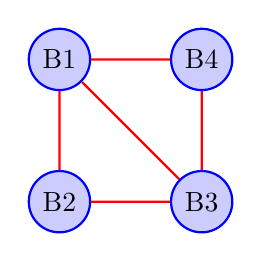
\begin{tikzpicture}
            \node [inner,draw=blue] (bi)  {B1};
            \node [inner,draw=blue,below=of bi] (bii) {B2};
            \node [inner,draw=blue,right=of bii] (biii) {B3};
            \node [inner,draw=blue,right=of bi] (biv) {B4};
            \draw[red,thick] (bi) -- (bii) -- (biii) -- (biv) -- (bi) -- (biii);
        \end{tikzpicture}
    };
    \draw[thick,orange,->] (ai) -- (bii);
    \draw[orange,->] (aiii) -- (bi);
    \draw[orange,->] (A.90) -- ($(A.90)+(0,1)$) -| (B);
\end{tikzpicture}
\end{document}
